\chapter{Eksperimentel opstilling og metoder}
\label{chap:methods}

\section{Overordnet valideringsstrategi}
Projektets eksperimentelle del bestod af tre komplementære spor. Det analoge pulsoximetersystem udgjorde hovedsporet og blev anvendt til at måle PPG-signaler i transmissionsgeometri. Herudover blev et hyperspektralt setup anvendt som optisk valideringsspor til at undersøge den relative transmission gennem fingervæv ved udvalgte bølgelængder, mens et spektrometer blev anvendt til spektral karakterisering af de anvendte lyskilder og til supplerende transmissionsmålinger.

De tre spor havde således forskellige roller i projektet. Det analoge system blev brugt til at demonstrere den praktiske måling af PPG-signaler, mens de to optiske opstillinger blev anvendt til at understøtte og nuancere bølgelængdevalget samt verificere de anvendte lyskilders faktiske spektrale egenskaber.

\section{Analog måleopstilling}
\label{sec:analog_setup}

\subsection{Formål}
Formålet med den analoge opstilling var at undersøge, om det udviklede system kunne måle et brugbart PPG-signal i fingertransmission ved brug af rødt og nær-infrarødt lys. Derudover var formålet at vurdere, om signalet havde tilstrækkelig kvalitet til udtræk af puls og videre analyse af AC- og DC-komponenter.

\subsection{Fysisk opstilling}
Den analoge måleopstilling bestod af et 3D-printet kabinet/hylster med to LED'er og en fotodiode placeret over for hinanden, således at en finger kunne placeres mellem lyskilde og detektor. LED'erne blev styret via et separat driverkredsløb, mens det transmitterede lys blev detekteret af fotodioden og ført videre til den analoge signalkæde bestående af en transimpedansforstærker, filtrering og et afsluttende forstærkertrin.

Signalet blev opsamlet med et Analog Discovery 3, som både blev anvendt til styring af tidsmultipleksingen og til dataopsamling. Under måling blev den venstre pegefinger placeret i kabinettet med neglesiden vendt mod LED'erne og fingerblommen mod fotodioden. Kabinettet blev lukket omkring fingeren for at fastholde målegeometrien og reducere påvirkning fra omgivende lys. En elastik blev desuden placeret omkring top- og bunddelen for at fastholde fingerens placering.

De vigtigste komponenter i den analoge opstilling er opsummeret i tabel \ref{tab:centrale_komponenter}.

\begin{table}[h]
\centering
\caption{Centrale komponenter i det analoge system.}
\label{tab:centrale_komponenter}
\begin{tabular}{lll}
\toprule
Komponenttype & Valgt komponent & Funktion \\
\midrule
Fotodiode & Hamamatsu S1223 & Detektion af transmitteret lys \\
Operationsforstærker & OP27G & Transimpedansforstærker, filtrering og forstærkning \\
Rød LED & 660 nm LED & Hovedmåling i rød kanal \\
IR-LED & 940 nm LED & Hovedmåling i NIR-kanal \\
MOSFET & 2N7000 & Switching i LED-driver \\
Dataopsamling & Analog Discovery 3 & Styring og signalopsamling \\
\bottomrule
\end{tabular}
\end{table}

\subsection{Måleprotokol} 
Målingerne blev udført siddende, loftbelysning slukket og så stille som muligt, hurtigere eller dybe vejrtrækninger var undgået. Målingen var udført over et minut, med en initiel start-up forsinkelse på 15 sekunder, så forsøgspersonen kunne nå at placere fingeren stabilt i hylsteret før dataopsamlingen begyndte.

Derefter blev systemet kørt i 10 sekunder før dataopsamling for at lade LED-driver, analogkæde og softwaresekvens stabilisere sig. Til sidst blev der udført en minut lang måling, med en multipleksing frekvens på \SI{7.41}{Hz}.

\paragraph{Frekvensvalg.} Da man ønsker at måle et heltals multiplum af \SI{20}{ms}, kan man f.eks. vælge at måle hver af de tre faser, som vist i tabel \ref{tab:maalinger}, med tiden \SI{40}{ms}.

Hver målecyklus bestod af tre faser: \SI{660}{nm}-LED tændt, \SI{940}{nm}-LED tændt og begge LED'er slukket. Hver fase bestod af en settlingperiode på \SI{5}{ms} efterfulgt af et målevindue på \SI{40}{ms}. En komplet cyklus varede derfor
\begin{equation}
    T_{\mathrm{cyklus}} = 3 \cdot (\SI{5}{ms}+\SI{40}{ms}) = \SI{135}{ms},
\end{equation}
svarende til en kanalrate på
\begin{equation}
    f_{\mathrm{kanal}} = \frac{1}{T_{\mathrm{cyklus}}} \approx \SI{7.41}{Hz}
\end{equation}

Nyquist-kriteriet skal også overholdes, og da:
\begin{equation}
    120 \ \text{BPM} = 2 \ \text{Hz}
\end{equation}
og da Nyquist frekvensen er:
\begin{equation}
    \frac{7.41}{2} = 3.7 \ \text{Hz}
\end{equation}
Dækkes \SI{2}{Hz} komfortabelt.

Frekvensen var desuden valgt ud fra antagelsen at for en ren sinusformet \SI{50}{Hz}-komponent vil midlingen ideelt give nul middelværdi, man kan derfor fjerne støjen i software uden for stor byrde af lavpasfilteret, mere om lavpasfilter løsningen efter.

Løsningen for attenuering af \SI{50}{Hz} støjen bygger som sagt på antagelsen om, at støjen kan modelleres som en sinusformet forstyrrelse med ukendt fase $\varphi$. Middelværdien over et tidsvindue $T$ er:

\begin{equation}
    \frac{1}{T} \int_0^T A \sin (2 \pi \cdot 50 \cdot t + \varphi)\, dt = \frac{A}{2\pi \cdot 50 \cdot T} \cdot \left[\cos(\varphi) - \cos(2\pi \cdot 50 \cdot T + \varphi)\right]
\end{equation}

Hvis $T = \frac{N}{50 \ \text{Hz}}$ , hvor N er et positivt heltal svarende til et heltalligt multiplum af nettets periode $\frac{1}{50 \ \text{Hz}} = 20 \ \text{ms}$, gælder det at $2\pi \cdot 50 \cdot T = 2\pi N$, og dermed:
\begin{equation}
    \cos(2\pi N + \varphi) = \cos(\varphi)
\end{equation}

Dermed bliver de to cosinusled identiske, og middelværdien bliver nul uanset amplitude og fase.

\subsection{Elektrisk karakterisering}
I dette delafsnit vises plots med pulsoximeteret drevet ved \SI{7.41}{Hz}.

\paragraph{Transimpedance Amplifier - TIA}
TIA'en fungerede som både en konvertering fra strøm til spænding og en initiel forstærkning af det indkommende signal. Forstærkningen bestemmes ud fra feedbackmodstanden, $R_f$. Desuden er tilsat en kondensator, $C_f$, i parallel til $R_f$ for at hjælpe med hurtigt skiftende diodestrøm. De er sat til:

\begin{itemize}
    \item $C_f = 10 \ \text{pF}$
    \item $R_f = 2.21 \ \text{M}\Omega$
\end{itemize}

Ud fra TIA outputtet i resultatsafsnittet figur \ref{fig:TIA_output}, kan de omtrentlige middelværdier for de tre faser estimeres som:
\begin{itemize}
    \item $940 \ \text{nm} \ \xrightarrow{\text{Gennemsnit}} 0.9 \ \text{V}$
    \item $660 \ \text{nm} \ \xrightarrow{\text{Gennemsnit}} 0.5 \ \text{V}$
    \item $\text{Mørke} \ \xrightarrow{\text{Gennemsnit}} 0 \ \text{V}$
\end{itemize}

Størrelsen af den tilsvarende inputstrøm kan estimeres fra TIA-relationen
\[
    |I_{\text{in}}|=\frac{|V_{\text{out}}|}{R_f}.
\]
Med $R_f=2.21\,\text{M}\Omega$ fås omtrent
\[
    |I_{940}|=\frac{0.9}{2.21\cdot 10^6}=0.41\,\mu\text{A},
\]
og
\[
    |I_{660}|=\frac{0.5}{2.21\cdot 10^6}=0.23\,\mu\text{A}.
\]
Fotostrømmen i den analoge opstilling ligger dermed i størrelsesordenen $0.2$--$0.4\,\mu\text{A}$.

\paragraph{Lavpasfilter - LPF}
Lavpasfilteret er et andenordens Sallen-Key filter med følgende komponentværdier:
\begin{itemize}
    \item To modstande på $1 \ \text{M}\Omega$
    \item To kondensatorer på $1 \ \text{nF}$
    \item $f_{\text{knæk}} = \dfrac{1}{2\pi RC} \approx \SI{159}{Hz}$
\end{itemize}

Knækfrekvensen på \SI{159}{Hz} er bevidst placeret over PPG-signalets nyttige
båndbredde, men lavt nok til at begrænse den samlede støjbåndbredde i signalkæden inden sampling. Filteret har to primære funktioner:

\begin{enumerate}
    \item \textbf{Anti-aliasing for AD3'ens sampling.} AD3'en sampler kontinuerligt under hver \SI{40}{ms} LED-fase ved \SI{20}{kHz}, og prøverne midles efterfølgende til en værdi per fase. LPF'en bidrager til at dæmpe højfrekvent indhold over Nyquist-frekvensen på \SI{10}{kHz} inden digitalisering. 

Med en knækfrekvens på \SI{159}{Hz} og en rolloff på \SI{-40}{dB/dekade} er dæmpningen ved \SI{10}{kHz} på størrelsesordenen $10^{-4}$, hvilket reducerer risikoen for aliasing af højfrekvent støj.

    \item \textbf{Dæmpning af bredspektret højfrekvent støj.} Elektromagnetisk støj fra omkringliggende udstyr (skærme, strømforsyninger, switching elektronik) kan koble ind på JST-XH-kablingen og fotodiodens ledninger. Disse bidrag dæmpes effektivt af filteret.
\end{enumerate}

Den efterfølgende midling af samples inden for hver \SI{40}{ms} LED-fase udgør et lavpasfilter. Det første nul ligger ved $\frac{1} {T_{\text{fase}}} = \SI{25}{Hz}$, og \SI{50}{Hz} falder nær det andet nul. Midlingen undertrykker derfor \SI{50}{Hz}-støj fra elnettet markant, hvilket forklarer hvorfor analog \SI{50}{Hz}-filtrering ikke er nødvendig i signalkæden. LPF'en ved \SI{159}{Hz} dæmper \SI{50}{Hz} med en faktor:
\begin{equation}
    |H(\SI{50}{Hz})| = \frac{1}{\sqrt{1+\left(\frac{50}{159}\right)^4}}
    \approx 0.995
\end{equation}
altså med lav attenuation, \SI{50}{Hz} undertrykkelsen kommer fra midlingen i software, ikke fra analogfilteret. En lavere analog knækfrekvens ville desuden være upraktisk, da den ville kræve aflodning af de eksisterende \SI{1}{nF}-kondensatorer med tilhørende risiko for termisk skade på PCB'en. Resterende DC og langsom drift fra ambient-lys reduceres efterfølgende via mørkesubtraktion i software, som beskrevet i \cref{sec:signalbehandling}.

Effekten af LPF-trinnet er illustreret i resultat afsnittet i figur \cref{fig:LPF_output}, hvor det glattere signal efter LPF sammenlignet med TIA-udgangen i figur \ref{fig:TIA_output} viser dæmpningen af bredspektret højfrekvent indhold.

\paragraph{Højpas filter - HPF}
Højpasfilteret blev designet og produceret, men blev ikke anvendt i den endelige SpO$_2$-analyse, da beregningen af $AC/DC$ kræver adgang til DC-komponenten. Filteret var oprindeligt tænkt til at dæmpe DC-offset og meget langsom drift.

Filteret var dimensioneret med to modstande på $330\,\text{k}\Omega$ og to kondensatorer på $1\,\mu\text{F}$, hvilket giver en knækfrekvens på
\[
    f_{\text{knæk}}=\frac{1}{2\pi RC}
    =\frac{1}{2\pi\cdot 330\cdot 10^3\cdot 1\cdot 10^{-6}}
    \approx 0.48\,\text{Hz}.
\]
Denne frekvens svarer til cirka 29 BPM. Ved knækfrekvensen dæmpes signalet med 3 dB, mens højere pulsfrekvenser passerer med mindre dæmpning.

\paragraph{Ikke-inverterende forstærkning - Gain}
Gain stadiet havde følgende komponentværdier:
\begin{itemize}
    \item  En modstand på $R_f = 39 \ k \Omega$
    \item En modstand på $R_g = 10 \ k \Omega$
\end{itemize}

Som producerer en gain på:

\begin{equation}
    \text{Gain} = 1 + \frac{R_f}{R_g} = 1 + \frac{39000}{10000} = 4.9
\end{equation}

Den ikke inverterende forstærkning fungerede som det sidste stadie inden dataopsamling, og flyttede signalet ind i et område så ADC’ens dynamiske område blev udnyttet bedre.

\subsection{Signalbehandling}
Signalbehandlingen havde tre formål: demultipleksering af LED-kanalerne, estimering af puls og beregning af $\frac{AC}{DC}$-forhold til SpO$_2$-estimat.

\paragraph{Tidsdemultipleksering.}
Hver cyklus blev opdelt i tre faser: \SI{660}{nm}-LED tændt, \SI{940}{nm}-LED tændt og begge LED'er slukket. Hver fase bestod af \SI{5}{ms} settling efterfulgt af et \SI{40}{ms} målevindue. Settlingperioden blev kasseret i analysen, mens prøverne i målevinduet blev midlet til en værdi for den pågældende fase. En komplet cyklus tog derfor \SI{135}{ms}, svarende til en effektiv kanalrate på \SI{7.41}{Hz}.

\paragraph{Pulsestimat.}
I livevisningen blev pulsen estimeret med et glidende vindue på \SI{60}{s}. Da de analyserede optagelser varede \SI{60}{s}, svarer den endelige pulsværdi dog reelt til et estimat over hele målevinduet. Inden for vinduet fjernes en lineær trend (en ret linje fittes og trækkes fra), hvorved langsom drift i baseline ikke forstyrrer detektionen. Det trendfjernede signal glattes med et 0.35\,s middelvindue, og \texttt{scipy.signal.find\_peaks} finder lokale toppe med en mindste afstand svarende til \SI{140}{BPM} og en prominens på 30\% af peak-to-peak. Prominensen er, hvor højt en top rager op over det laveste niveau før en endnu højere top, og forhindrer at små ripler tælles som selvstændige slag. Algoritmen kører på både toppe og dale, og det sæt med mindst spredning på interbeat-intervallerne (tiderne mellem efterfølgende slag) vælges. Pulsen rapporteres som $\frac{60}{\tilde{T}_{\text{IBI}}}$, og estimater med relativ spredning over 35\% eller uden for 40 til \SI{140}{BPM} kasseres.

\paragraph{SpO\textsubscript{2}-estimat.}
I et \SI{30}{sek} vindue tages DC som signalets middelværdi, mens AC isoleres
med et nulfase Butterworth-båndpas af anden orden i hjertebåndet 0.5 til \SI{2}{Hz} (30 bpm til 120 bpm). AC-amplituden estimeres robust som forskellen mellem 95.- og 5.-percentilen, hvilket dæmper enkeltstående bevægelsesartefakter. Forholdet
\begin{equation}
\label{eq:ratio_of_ratios}
  R = \frac{\frac{AC_{660}}{DC_{660}}}{\frac{AC_{940}}{DC_{940}}}
\end{equation}
omsættes til iltmætning via en lineær kalibrering $\mathrm{SpO_2} = a - bR$, hvor $a$ og $b$ bestemmes mod et kommercielt pulsoximeter anvendt som praktisk reference, kalibreringen beskrives i resultatafsnittet. Værdier med for lav DC, for lav AC-amplitude eller fysiologisk urealistisk SpO$_2$-estimat blev markeret som ugyldige.

\subsection{Udledte parametre}
Fra de demultipleksede og mørkekorrigerede signaler blev følgende parametre udledt:
\begin{itemize}
    \item $V_{660}(t)$ og $V_{940}(t)$: mørkekorrigerede tidsserier for de to LED-kanaler.
    \item $DC_{660}$ og $DC_{940}$: middelværdien af signalerne i analysevinduet.
    \item $AC_{660}$ og $AC_{940}$: pulsatile amplituder estimeret efter båndpasfiltrering.
    \item $R$: ratio-of-ratios beregnet som vist i ligning \ref{eq:ratio_of_ratios}
    \item Puls: estimeret fra interbeat-intervaller i \SI{940}{nm}-kanalen.
    \item SpO$_2$: proof-of-concept-estimat beregnet via en empirisk lineær kalibrering.
\end{itemize}

\section{Hyperspektral opstilling}
\label{sec:hyperspectral_setup}

\subsection{Formål}
Formålet med den hyperspektrale opstilling var at undersøge den relative detekterede intensitet gennem en finger ved udvalgte nær-infrarøde bølgelængder. Målingen blev ikke anvendt som et selvstændigt pulsoximeter, men som et optisk valideringsspor til at vurdere, hvilke bølgelængdeområder der gav brugbare signalniveauer under den givne transmissionsgeometri.

Da den målte intensitet afhænger af både vævstransmission, lyskildens spektrum, filterets transmission, linsernes transmission og kameraets kvanteeffektivitet, fortolkes resultaterne som relative målinger for den konkrete opstilling og ikke som absolutte vævstransmissioner.

\subsection{Opstilling}
Den hyperspektrale opstilling bestod af en bredbåndet Glo-bar som infrarød lyskilde, en fingerholder, et linsehus med tre akromatiske dubletter, et lineært variabelt filter (LVF), en lineær stage og et NIR-følsomt kamera. Kameraet var et UI-3240CP-NIR-GL, som har forhøjet følsomhed i det nær-infrarøde område sammenlignet med et almindeligt synligt kamera.

Glo-baren blev anvendt som transmissionslyskilde. Fingeren blev placeret i strålegangen mellem lyskilden og det optiske detektionssystem. Det transmitterede lys fra fingeren blev opsamlet af linseopstillingen og sendt videre mod LVF'et og kameraet. LVF'et fungerede som et positionsafhængigt båndpasfilter, hvor den transmitterede centerbølgelængde afhænger af filterets position. Ved at flytte LVF'et med den lineære stage kunne forskellige smalle spektrale bånd selekteres sekventielt.

Mellem fingerpositionen og LVF'et var et linsehus monteret med tre akromatiske dubletter. Den første linse var en akromatisk dublet med fokalllængde på 30 mm og diameter på 1 inch, mens de to efterfølgende linser havde fokallængder på henholdsvis 50 mm og 25 mm og diameter på 1/2 inch. Alle linser havde antirefleksbelægning(ARC) specificeret til området 400-1100 nm.

Linsernes funktion var at opsamle og forme det transmitterede lys fra fingeren, så en brugbar del af lyset kunne føres videre gennem LVF'et og registreres på kameraet. Den store linse nærmest fingeren opsamlede en større del af det transmitterede lysfelt, mens de efterfølgende linser indgik i den videre afbildning mod filter og kamera.

Afstandene mellem de enkelte optiske komponenter blev justeret praktisk for at opnå et klart og reproducerbart billede på kameraet. Da opstillingen ikke var designet som et fuldt radiometrisk kalibreret billeddannende system, blev analysen baseret på relativ intensitet i en fast ROI og efterfølgende spektral korrektion.

\begin{figure}[htbp]
    \centering
    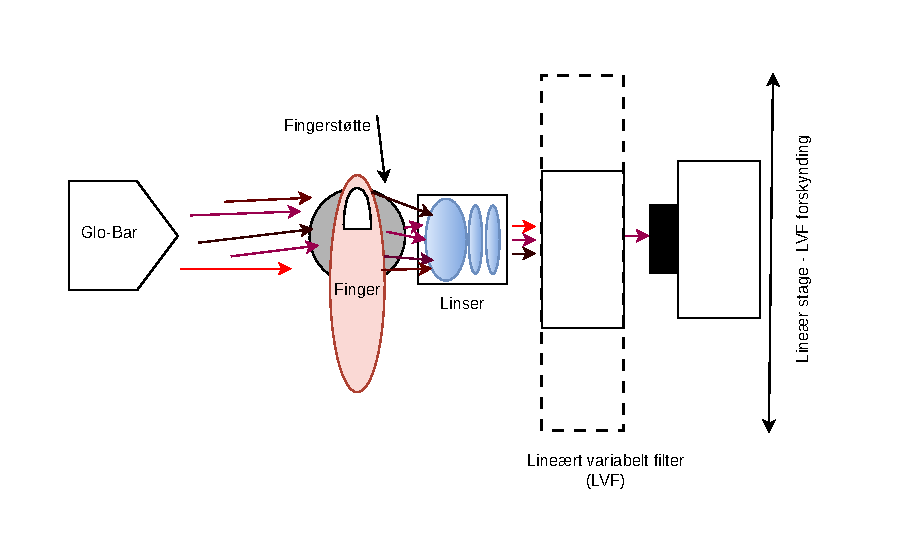
\includegraphics[width=1\textwidth]{Pictures/Other/Hyperspektral_diagram.pdf}
    \caption{Hyperspektral transmissionsopstilling. En Glo-bar anvendes som bredbåndet infrarød lyskilde, og det transmitterede lys gennem fingeren føres gennem linser, et lineært variabelt filter (LVF) og registreres af et NIR-følsomt kamera. Ved horisontal forskydning af LVF'et ændres det transmitterede spektrale bånd, således at forskellige bølgelængdeområder kan måles sekventielt.}
    \label{fig:hyperspekt_diagram}
\end{figure}

\subsection{Måleprocedure}
Den hyperspektrale opstilling blev anvendt til at undersøge bølgelængder nær 810 nm og 940 nm. Bølgelængden 660 nm blev ikke inkluderet, da LVF'et ikke dækkede dette område. Følgende bølgelængder blev undersøgt:

\begin{itemize}
    \item 800 nm
    \item 810 nm
    \item 820 nm
    \item 930 nm
    \item 940 nm
    \item 950 nm
\end{itemize}

For hver bølgelængde blev LVF'et flyttet til den tilsvarende position på den lineære stage ud fra en tidligere bestemt kalibreringskurve mellem stageposition og peak-bølgelængde. Billederne blev optaget med ThorCam-softwaren på en tilkoblet laptop. Integrationstid, kameraindstillinger og optisk geometri blev holdt konstante gennem måleserien for at gøre pixelintensiteterne sammenlignelige.

Før måleserien blev der optaget mørkebilleder med samme kameraindstillinger som fingerbillederne. Under målingerne blev loftbelysning og andre direkte lyskilder i lokalet slukket eller vendt væk fra opstillingen for at reducere bidrag fra omgivelseslys. Fingeren blev så vidt muligt holdt i samme position for alle bølgelængder, så ændringer i målt intensitet primært skyldtes ændret bølgelængde og ikke ændret målegeometri.

Referencebilleder uden finger blev ikke anvendt til direkte normalisering, da intensiteten uden finger var væsentligt højere end med finger og kunne give mætning ved samme integrationstid. I stedet blev fingerbillederne mørkekorrigeret og derefter korrigeret med kendte spektrale bidrag fra Glo-bar, linser, LVF og kamera.

\subsection{Opløsning og valg af ROI}
\label{resolution_ROI}
LVF'et har en endelig spektral båndbredde. Den iboende båndbredde for filteret var cirka 10 nm FWHM. Derudover bidrager den optiske afbildning til en mindre udtværing af bølgelængder, fordi et fokuseret lyspunkt på LVF'et dækker et lille interval af filterpositioner. For et fokuseret spot på cirka 0.19 mm og en LVF-gradient på 17.05 nm/mm bliver det spatiale bidrag

\begin{equation}
    \Delta \lambda_{\mathrm{spatial}}
    =
    0.19\,\mathrm{mm}
    \cdot
    17.05\,\frac{\mathrm{nm}}{\mathrm{mm}}
    \approx
    3.24\,\mathrm{nm}.
\end{equation}
Der kan desuden forekomme et mindre vinkelafhængigt bidrag, fordi LVF'ets transmissionsbånd afhænger af indfaldsvinklen. Dette bidrag afhænger af keglen af stråler ved filteret og blev derfor behandlet som en metodisk usikkerhed i størrelsesordenen af få nanometer.

Da LVF'et har en bølgelængdegradient, kan et bredt ROI dække flere peak-bølgelængder på en gang. ROI'et blev derfor valgt smalt i den retning, hvor bølgelængden varierer mest, og højt i den lodrette retning. Denne strategi reducerer udtværing af bølgelængder, samtidig med at et tilstrækkeligt antal pixels bevares til beregning af pixelintensitet.

\subsection{Billedanalyse og spektral korrektion}
Formålet med billedanalysen var at estimere fingerens relative, spektralt korrigerede transmission ved de udvalgte bølgelængder.

\begin{figure}[htbp]
    \centering
    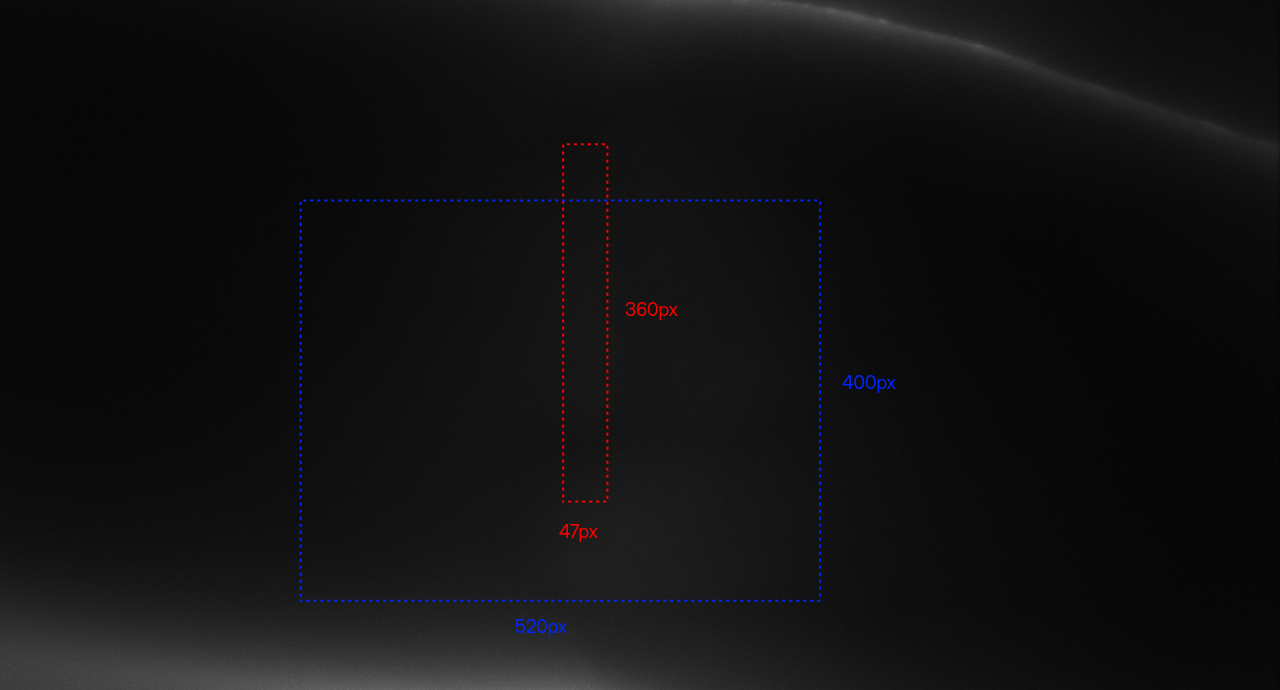
\includegraphics[width=1\textwidth]{Pictures/Other/finger_930nm_roi_regioner.png}
    \caption{Figuren viser to indtegnede ROIs, den første, brede region (520x400px) og den efterfølgende smalle region (47x360px).}
    \label{fig:roi_zoom}
\end{figure}

For hver bølgelængde blev fingerbilledet og det tilhørende mørkebillede først læst ind. Mørkebillederne havde oprindeligt dimensionerne 1280 x 1024 pixels, mens fingerbillederne havde dimensionerne 1280 x 690 pixels. Mørkebillederne blev derfor centreret beskåret med 167 pixels fra top og bund, så mørke- og fingerbilleder fik samme dimensioner. Herefter kunne samme ROI-koordinater anvendes direkte i begge billeder.

Den mørkekorrigerede pixelintensitet blev beregnet som

\begin{equation}
    I_{\mathrm{korr}}(x,y,\lambda)
    =
    I_{\mathrm{finger}}(x,y,\lambda)
    -
    I_{\mathrm{mørke}}(x,y,\lambda)
\end{equation}

For hver bølgelængde blev der udvalgt en fast ROI centralt på fingeren. ROI'et blev placeret væk fra fingerens kanter, da randregionerne var præget af Fresnelrefleksioner. Disse randbidrag blev ikke betragtet som repræsentative for transmission gennem fingerens væv.

For hver bølgelængde blev der beregnet både median og gennemsnit af den mørkekorrigerede intensitet i ROI'et. Medianen blev anvendt som primær statistik, mens gennemsnittet blev anvendt som kontrol.\begin{equation}
    I_{\mathrm{median}}(\lambda)
    =
    \operatorname{median}_{ROI}
    \left[
    I_{korr}(x,y,\lambda)
    \right]
\end{equation}
\begin{equation}
    I_{\mathrm{mean}}(\lambda)
    =
    \operatorname{mean}_{ROI}
    \left[
    I_{korr}(x,y,\lambda)
    \right]
\end{equation}

Den målte intensitet kan beskrives som proportional med produktet af flere spektrale led:
\begin{equation}
    I_{\mathrm{målt}}(\lambda)
    \propto
    E_{\mathrm{glo-bar}}(\lambda)
    \cdot
    T_{\mathrm{finger}}(\lambda)
    \cdot
    T_{\mathrm{linser}}(\lambda)
    \cdot
    T_{\mathrm{filter}}(\lambda)
    \cdot
    QE_{\mathrm{kamera}}(\lambda)
    \cdot
    \lambda
\end{equation}
Faktoren $\lambda$ indgår, fordi Glo-barens spektrum er angivet i energi-enheder, mens kameraets quantum efficiency angiver sandsynligheden for ladningsbærergeneration per indfaldende foton. For samme optiske effekt er antallet af fotoner proportionalt med bølgelængden.

Fingerens relative, spektralt korrigerede signal blev derfor estimeret som

\begin{equation}
    F_{\mathrm{korr}}(\lambda)
    =
    \frac{
    I_{\mathrm{målt}}(\lambda)
    }
    {
    E_{\mathrm{glo-bar}}(\lambda)
    \cdot
    T_{\mathrm{linse1}}(\lambda)
    \cdot
    T_{\mathrm{linse2}}(\lambda)
    \cdot
    T_{\mathrm{linse3}}(\lambda)
    \cdot
    T_{\mathrm{filter}}(\lambda)
    \cdot
    QE_{\mathrm{kamera}}(\lambda)
    \cdot
    \lambda
    }
\end{equation}
Da den absolutte koblingseffektivitet og geometri ikke var kendt, blev signalet normaliseret til 940 nm:
\begin{equation}
    T_{\mathrm{finger,rel}}(\lambda)
    =
    \frac{
    F_{\mathrm{korr}}(\lambda)
    }
    {
    F_{\mathrm{korr}}(940\,\mathrm{nm})
    }
\end{equation}
Denne størrelse beskriver den relative, spektralt korrigerede transmission gennem fingeren i den givne opstilling. Den skal derfor ikke fortolkes som en absolut vævstransmission, men som et sammenligningsmål mellem de undersøgte bølgelængdeområder.

De spektrale korrektionsfaktorer for Glo-bar, linser, LVF og kameraets kvanteeffektivitet er samlet i appendiks~\ref{tab:hyperspectral_correction_values}. Disse værdier blev anvendt til beregning af den relative, spektralt korrigerede fingertransmission.

\subsection{Begrænsninger}
Den hyperspektrale opstilling havde flere metodiske begrænsninger:

\begin{itemize}
    \item Målingen var sekventiel og ikke synkroniseret til hjerteslaget. Billeder ved forskellige bølgelængder kan derfor være optaget ved forskellige faser af pulsen, hvilket kan påvirke den målte intensitet gennem ændret blodvolumen i fingeren.

    \item Den spektrale korrektion bygger på databladsværdier og målte eller estimerede transmissionskonstanter for de enkelte optiske led. Usikkerheder i Glo-barens spektrum, linsetransmission, LVF-transmission og kameraets kvanteeffektivitet påvirker derfor den korrigerede relative transmission.

    \item LVF'et har en endelig spektral båndbredde. Den effektive båndbredde blev estimeret til omkring 11 nm og domineres af filterets iboende FWHM på cirka 10 nm. De rapporterede bølgelængder skal derfor forstås som nominelle centerbølgelængder for smalle spektrale bånd, ikke som ideelt monokromatiske målinger.

    \item LVF'et dækkede ikke 660 nm. Den røde pulsoximetrikanal kunne derfor ikke undersøges med denne opstilling. Den hyperspektrale opstilling blev primært anvendt til at sammenligne nærliggende NIR-bølgelængder omkring 810 nm og 940 nm.

    \item Vignettering, små ændringer i fingerplacering og ufuldstændig reproducerbarhed af ROI-positionen kan påvirke de målte intensiteter. Disse effekter blev reduceret ved at anvende en fast central ROI, mørkekorrektion og normalisering til 940 nm.
\end{itemize}

\section{Spektrometrisk karakterisering}
\label{sec:spectrometer_characterization}

\subsection{Formål}
Formålet med den spektrometriske karakterisering var at verificere de faktiske spektrale egenskaber for de anvendte lyskilder. Spektrometeret blev primært anvendt til at bestemme peak-bølgelængde og spektral bredde for LED-kandidaterne, til at sammenligne de indkøbte LED’er med et kommercielt pulsoximeter og til at karakterisere Glo-barens spektrale fordeling som input til den hyperspektrale korrektion.

Der blev desuden udført en orienterende transmissionsmåling gennem pegefingeren med en bredbåndskilde. Denne måling blev ikke anvendt som kvantitativ vævstransmission, da der ikke blev optaget en tilsvarende reference uden finger under samme geometri og integrationstid. Målingen blev derfor kun brugt kvalitativt til at vurdere, om der var målbart lys efter passage gennem fingeren.

\subsection{Opstilling}
Spektrometermålingerne blev udført med en fiberkoblet spektrometerprobe monteret i et stativ på det optiske bord. Proben blev holdt i en fast position under hver måleserie for at reducere variationer fra geometri og afstand. Ved måling af LED’er blev lyskilden placeret i en reproducerbar afstand fra proben, cirka 10 cm, og orienteret mod probens optiske akse.

Ved måling af bredbåndskilder blev proben placeret, så spektrometeret opsamlede lyset fra kilden under en fast geometri. Ved den orienterende fingertransmissionsmåling blev pegefingeren placeret mellem bredbåndskilden og proben, så spektrometeret registrerede det lys, der passerede gennem fingeren.

For hver måleserie blev der optaget et mørkespektrum med samme integrationstid som de tilhørende målinger. Mørkespektret blev trukket fra i den efterfølgende analyse.

\begin{figure}[htbp]
    \centering
    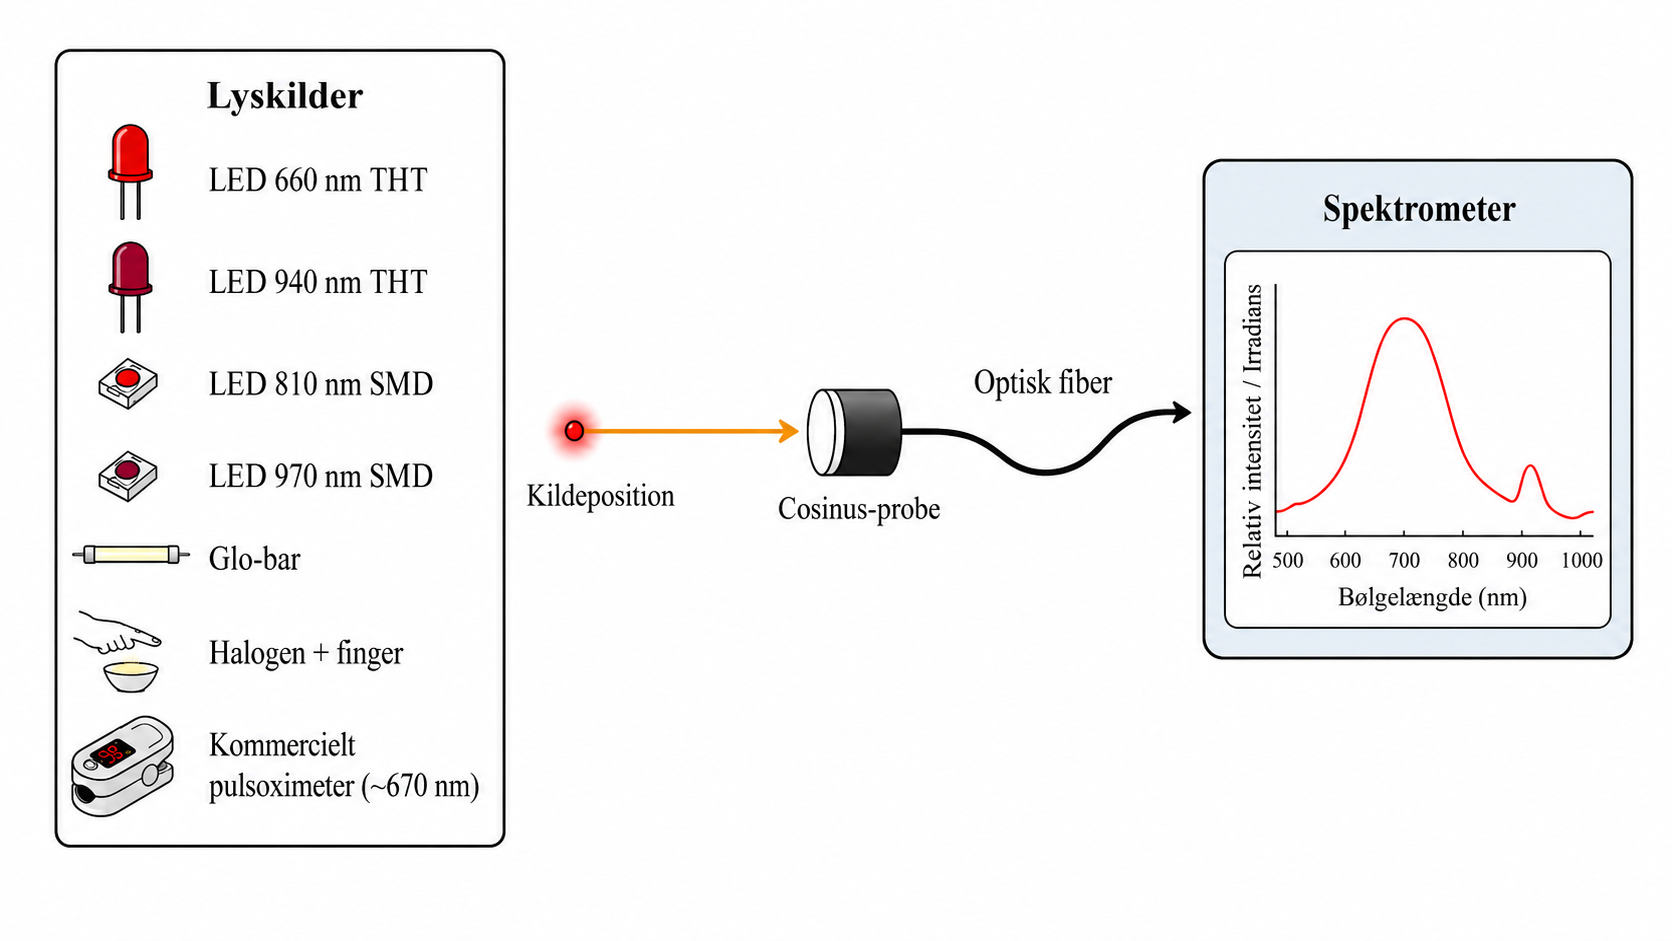
\includegraphics[width=1\textwidth]{Pictures/Other/Spektrometer_diagram.png}
    \caption{Spektrometeropstilling anvendt til spektral karakterisering af LED’er, bredbåndskilder og en orienterende fingertransmissionsmåling. Spektrometeret blev primært anvendt som valideringsværktøj til at bestemme lyskildernes faktiske spektrale egenskaber.}
    \label{fig:spektro_diagram}
\end{figure}

\subsection{Måleprocedure}

Følgende lyskilder og målesituationer blev karakteriseret:

\begin{itemize}
    \item 660 nm THT-LED
    \item 940 nm THT-LED
    \item 810 nm SMD-LED
    \item 970 nm SMD-LED
    \item kommercielt Braun-pulsoximeter
    \item Glo-bar
    \item orienterende transmissionsmåling gennem pegefinger med bredbåndskilde
\end{itemize}

For hver måling blev integrationstiden valgt, så spektret ikke var mættet. Da forskellige lyskilder havde forskellig intensitet, blev integrationstiden ikke nødvendigvis holdt ens på tværs af alle målinger. Spektrene blev derfor ikke brugt til direkte sammenligning af absolut intensitet, medmindre integrationstid og målegeometri var ens. Når spektrenes form skulle sammenlignes, blev de mørkekorrigerede spektre normaliseret til deres egen maksimale intensitet.

Ved måling af det kommercielle pulsoximeter blev spektrometeret anvendt til at identificere de spektrale områder, som instrumentet udsendte lys i. Da pulsoximeteret tidsmultiplekser sine LED’er, blev målingen fortolket som en spektral karakterisering af de udsendte lyskilder og ikke som en tidsopløst måling.

Glo-barens spektrum blev anvendt som en del af den spektrale korrektion i den hyperspektrale analyse. Da den målte Glo-bar-intensitet afhænger af både lyskildens spektrum, spektrometerets respons og målegeometrien, blev værdierne anvendt som en relativ spektral korrektion for den konkrete opstilling.

\subsection{Dataanalyse}

For hver LED blev peak-bølgelængden bestemt som den bølgelængde, hvor det mørkekorrigerede spektrum havde maksimal intensitet. Spektralbredden blev bestemt ved full width at half maximum (FWHM), dvs. bredden af spektret ved halvdelen af maksimal intensitet.

For at sammenligne LED-kandidaternes spektrale form blev hvert LED-spektrum normaliseret til sit maksimum:

\begin{equation}
    I_{\mathrm{norm}}(\lambda)=
    \frac{
    I(\lambda)-I_{\mathrm{dark}}(\lambda)
    }
    {
    \max\left(I(\lambda)-I_{\mathrm{dark}}(\lambda)\right)
    }
\end{equation}

Denne normalisering fjerner forskelle i absolut intensitet forårsaget af afstand, vinkel, LED-effekt og integrationstid, men bevarer information om peak-bølgelængde og spektral bredde. De normaliserede spektre blev derfor anvendt til at verificere, om LED’erne lå tæt på de ønskede bølgelængder.

For Glo-bar-målingen blev det mørkekorrigerede spektrum anvendt til at beskrive den relative spektrale fordeling af den bredbåndede lyskilde i det relevante bølgelængdeområde. Dette spektrum blev senere anvendt som et korrektionsled i den hyperspektrale analyse.

Den orienterende fingertransmissionsmåling blev ikke anvendt til beregning af kvantitativ transmission. Uden en reference uden finger under samme geometri kan det målte spektrum ikke isolere fingerens transmission fra bredbåndskildens spektrum og spektrometerets spektrale respons. Målingen blev derfor kun brugt kvalitativt som en indikation af, at der kunne registreres lys efter passage gennem fingeren.